\section{Theorie}
\subsection{Der glühelektrische Effekt}
Die thermische Elektronenemission beschreibt das Lösen von freien Elektronen aus aufgeheizten Metallen.
Dieses Phänomen wird auch als \textbf{glühelektrischer Effekt} bezeichnet und ist durch die Ionisierung der Atome in Metallmolekülen möglich.
Dadurch entstehen freie Elektronen, die die kristalline, periodisch angeordnete Gittertruktur des Moleküls als Wolke umgeben und auch \textbf{Leitungselektronen} genannt werden.
Sie sind auch der Grund für die hohe elektrische und thermische Leitfähigkeit.
Näherungsweise kann von einem konstanten Gitterpotential ausgegangen werden.
Um das Elektron aus dem Metall zu lösen, müssen die Elektronen im Vergleich zum Vakuum aber eine materialabhängige Austrittsarbeit $e_0 \phi$ verrichten, da es sich in einem Potentialtopf, wie es in Abbildung \ref{fig:pot} gezeigt wird, befindet.
$\xi$ gibt dabei das zu überwindene elektrische Potential an.
\begin{figure}[h]
    \centering
    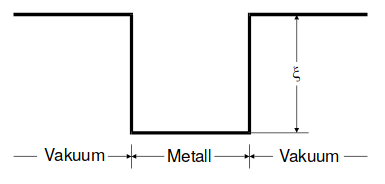
\includegraphics[height=4cm]{Theorie/Potentialtopf.png}
    \caption{Elektron im Potentialtopf.}
    \label{fig:pot}
\end{figure}

Die Wahrscheinlichtkeit dafür, dass Elektronen bestimmte Energiewerte im Metall annehmen, lässt sich durch die \textbf{Fermi-Diracsche Verteilungs-Funktion}
\begin{equation}
    \label{eqn:fermi}
    f (E) = \frac{1}{\text{exp} \left (\frac{E - \zeta}{\text{k}_\text{B} T} \right) + 1}
\end{equation}
beschrieben.
Dabei ist $f$ die Wahrscheinlichkeit, $E$ der Energiewert, $\zeta$ die fermische Grenzenergie und $k$ die Boltzmannkonstante.
Durch die Näherung $\zeta \gg kT$ bei Zimmertemperatur lässt sich die Gleichung auf
\begin{equation}
    \label{eqn:fermi2}
    f (E) \approx \text{exp} \left( \frac{\zeta - E}{\text{k}_\text{B} T}\right)
\end{equation}
bringen und wie in Abbildung \ref{fig:fermi} bei unterschiedlichen Temperaturen darstellen.
Die fermische Grenzenergie $\zeta$ gibt dabei die maximale Energie beim absoluten Temperaturnullpunkt an, die aufgrund der Quantentheorie und des Pauli-Prinzips erreicht wird.
Bei Temperaturen $T > 0$ gibt es also die Möglichkeit, dass Elektronen mit einer bestimmten Wahrscheinlichkeit Energien annehmen, die größer als die Austrittsarbeit sind, und sich somit aus dem Metall lösen.
Je höher also die Temperatur des Metalls, desto höher die Wahrscheinlichkeit, dass Elektronen Energien größer als die Austrittsarbeit annehmen.
\begin{figure}[h]
    \centering
    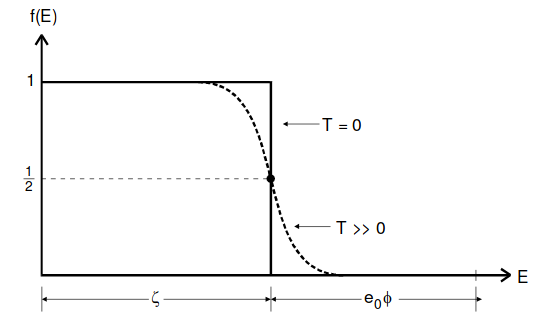
\includegraphics[height=4cm]{Theorie/Fermi.png}
    \caption{.Verlauf der Wahrscheinlichkeitsverteilung bei diskreten Energieniveaus}
    \label{fig:fermi}
\end{figure}
Aus der Gleichung \ref{eqn:fermi2} folgt nun die \textbf{Richardson-Gleichung}.
Für die Richardson-Gleichung und somit die Sättigungsstromdichte folgt schließlich durch Integration über den Impulsraum
\begin{equation}
    \label{eqn:rich}
    j_s (T) = 4\pi \frac{e_0 m_0 \text{k}_\text{B}^{2}}{h^{3}} T^{2} \text{exp} \left(\frac{-e_0 \phi}{\text{k}_\text{B} T}\right),
\end{equation}
wobei $e_0$ die Elementarladung, $m_0$ die Elektronenmasse und $\phi$ das Potential des Metalls darstellen.

\subsection{Die Hochvakkum-Diode}
Zur Messung der thermischen Elektronenemission wird eine Hochvakkum-Diode verwendet.
Dabei wird die Kathode, meist ein Metalldraht, über die Heizspannung auf Temperaturen von $1000 - 3000 K$ erhitzt, sodass sich Elektronen aus dem Metall lösen.
Des Weiteren wird eine Saugspannung zwischen Kathode und Anode angelegt, die die emittierten Elektronen aus der Kathode zur Anode absaugen.
Dadurch entsteht ein Anodenstrom, der die Elektronenemission nachweist.
Der ganze Vorgang muss im Vakuum stattfinden, da die emittierten Elektronen ansonsten mit den Gasmolekülen wechselwirken könnten und der Draht durchbrennen könnte.
\begin{figure}[h]
    \centering
    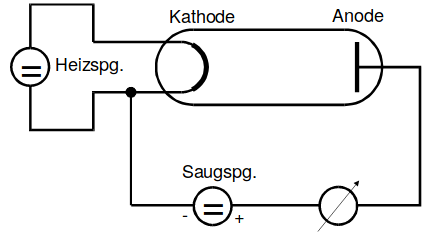
\includegraphics[height=4cm]{Theorie/Diode.png}
    \caption{.Beschaltung einer Hochvakkum-Diode}
    \label{fig:diode}
\end{figure}

\subsection{Die Langmuir-Schottkysche Raumladungsgleichung}
Über die Bestimmung des Anodenstroms nach Abbildung \ref{fig:diode} wird festgestellt, dass die Abhängigkeit des Anodenstroms zur Saugspannung erst bei hinreichend hoher Saugspannung verschwindet.
Bei niedrigen Spannungen erreichen nicht alle emittierten Elektronen die Anode.
Auf dem Weg zur Anode erfahren die Elektronen eine Beschleunigung, sie bewegen sich also nicht mit einer konstanten Geschwindigkeit fort.
Daraus lässt sich schließen, dass das Ohmsche Gesetz, also die Proportionalität von Spannung und Strom, in der Diode nicht gültig ist.
Außerdem kann aus der räumlich kontinuerlichen Stromdichte $ j = \rho \cdot v$ gefolgert werden, dass die Ladungsdichte neben der Geschwindigkeit ebenfalls nicht konstant ist und zur Anode hin abnimmt.
Dadurch wird das elektrische Feld der Kathode in Abhängigkeit der Ladungsdichte $\rho$ abgeschirmt und es ergibt sich ein kleinerer als nach Gleichung \ref{eqn:rich} zu erwartender Sättigungsstrom.
Um das Potential und das elektrische Feld quantitativ zu berechnen, wird die Potentialgleichung oder Poissonsche Gleichung
\begin{equation}
    \label{eqn:Poten}
    \Delta V = - \frac{1}{\epsilon_0} \rho
\end{equation}
als Ausgangspunkt verwendet.
Durch Umformungen und Erweiterungen ergibt sich für das Potential
\begin{equation}
    \label{eqn:Pot}
    \sqrt[4]{V^{3}} = \frac{3}{4} \sqrt{\frac{4j}{\epsilon_0 \sqrt{2e_0/m_0}}}\; x,
\end{equation}
wobei $x$ der Abstand zur Kathode ist und $V(0) = 0$ gilt.
Außerdem folt nach $E = -grad(V)$, dass sich die Feldstärke nach einem $\sqrt[3]{x^{4}}$-Gesetz ausbreitet.
Aus den Gleichungen \ref{eqn:Poten} und \ref{eqn:Pot} folgt für die Ladungsdichte eine $x^{-\frac{2}{3}}$-Abhängigkeit, was in Abbildung~\ref{fig:gebiet} für die essentiellen Größen dargestellt ist.
Zuletzt folgt als Gleichung für die Stromdichte
\begin{equation}
    \label{eqn:strom}
    j = \frac{4}{9} \epsilon_0 \sqrt{2 e_0/m_0} \frac{V^{\frac{3}{2}}}{a^{2}}, 
\end{equation}
welche auch als Langmuir-Schottkysche-Raumladungsgleichung bezeichnet wird.
Es wird deutlich, dass das Ohmsche Gesetz mathematisch auch seine Gültigkeit in der Hochvakkum-Diode verliert.
Das Gebiet, in welchem das Langmuir-Schottkysche-Raumladungsgesetz gilt, wird auch als Raumladungsgebiet definiert.

\begin{figure}[h]
    \centering
    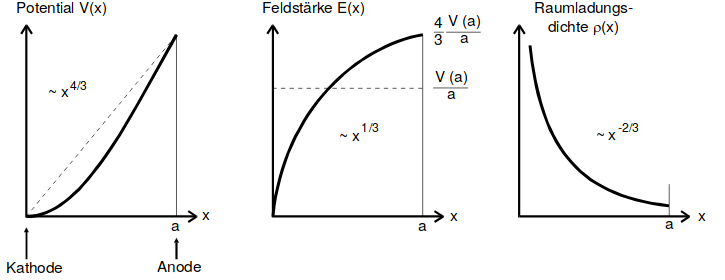
\includegraphics[height=4cm]{Theorie/Gebiet.png}
    \caption{.Ortsabhängigkeit des Potentials $V$, der Feldstärke $E$ und der Raumladungsdichte $\rho$ im Raumladungsgebiet einer Hochvakkum-Diode}
    \label{fig:gebiet}
\end{figure}

\subsection{Das Anlaufstromgebiet einer Hochvakuum-Diode}
Als Anlaufstrom wird der Strom bezeichnet, der bei $V = 0$ trotzdem gemessen werden kann, obwohl nach Gleichung \ref{eqn:strom} die Stromdichte dann ebenfalls verschwinden sollte.
Dieser entsteht durch die überschüssige Energie einiger Elektronen nach Abzug der Austrittnsarbeit $\phi$ und der fermischen Grenzenergie $\zeta$.
Der Energieüberschuss
\begin{equation}
    \label{eqn:energie}
    \Delta E = E - (\zeta + e_0 \phi)
\end{equation}
liefert die kinetische Energie für die emittierten Elektronen.
Dadurch ist es möglich, dass die Elektronen somit sogar gegen ein geringes Gegenfeld anlaufen können.
\begin{figure}[h]
    \centering
    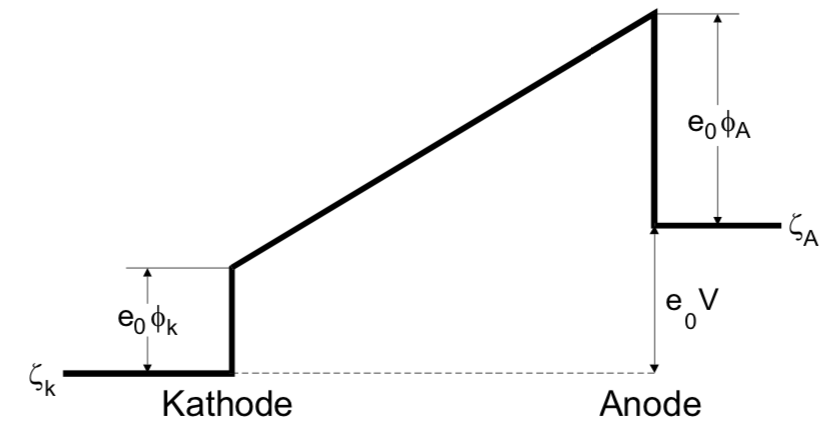
\includegraphics[height=4cm]{Theorie/Anlauf.png}
    \caption{.Das Anlaufstromgebiet mit den verschiedenen Energieniveaus bzw. Potentialen}
    \label{fig:anlauf}
\end{figure}
Die Abbildung \ref{fig:anlauf} zeigt, dass die Anode ebenfalls eine Austrittsarbeit besitzt.
Außerdem verschieben sich die fermischen Grenzenergien bei einer dazugeschalteten Spannung um $e_0 V$ zueinander.
Zusätzlich wird der Abbildung \ref{fig:anlauf} entnommen, dass Elektronen, die die Anode erreichen, eine Energie größer als $e_0 \phi_A + \zeta_A$ besitzen müssen. \\
Analog zur Bestimmung der Energie in Gleichung \ref{eqn:fermi2} wird die Abhängigkeit der Stromdicht vom angelegten Potential mit
\begin{equation}
    j(V) = j_0 \; \text{exp} \left (-\frac{e_0 \phi_\text{A} + e_0 V}{\text{k}_\text{B} \; T} \right) = \text{const.} \; \text{exp} \left ( - \frac{e_0 V}{\text{k}_\text{B} \; T}\right)
\end{equation}

\subsection{Die Kennlinie einer Hochvakuum-Diode}
Die Kennlinie der Hochvakkum-Diode beschreibt die Abhängigkeit des Anodenstroms $I_A$ von der angelegten Spannung $U$.
Es werden grundsätzlich drei verschiedene Gebiete der Kennlinie definiert.
Das Anlaufstromgebiet, welches im Bereich $V < 0$ liegt, lässt sich durch einen exponentiellen Zusammenhang kennzeichnen.
Die Kennlinie setzt sich dann in dem Raumladungsgebiet fort, welches eine $\sqrt{V^{3}}$-Abhängigkeit aufwei\ss{}t.
Dies folgt aus der Raumladungsgleichung \ref{eqn:strom}, welche aber noch von der Anodenspannung abhängt.
Der Anodenstrom hängt allerdings nicht von der Anodenspannung, sondern von der Temperatur, ab.
Nach der Richardson-Gleichung \ref{eqn:rich} geht der Anodenstrom aber einem Sättigungswert $I_S$ entgegen, da die Anzahl der auszulösenden Elektronen begrenzt ist.
Dadurch folgt auf das Raumladungsgebiet noch das Sättigungsstromgebiet.
Eine typische Kennlinie für eine gewählte Kathodentemperatur ist in Abbildung \ref{fig:kennlinie} dargestellt.

\begin{figure}[h]
    \centering
    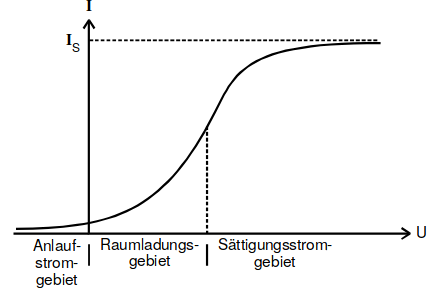
\includegraphics[height=4cm]{Theorie/Kennlinie.png}
    \caption{.Kennlinie einer Hochvakuum-Diode}
    \label{fig:kennlinie}
\end{figure}
